\chapter{Background}
\label{chap:background}

Before introducing the serverless paradigm,
we must understand what is cloud computing~\cite{nist}.
Despite its modern connotations, cloud computing
isn't a novel concept, in fact, its principles have been established
several decades ago: in essence, cloud computing
runs different types of workloads within clouds, which are environments that abstract, pool,
and share scalable resources across distributed networks.
Thus, users are offered on-demand availability of computing power by a third-party provider,
without the problems associated with direct active management of IT infrastructures.

\section{Cloud services}

Cloud computing is supplied as a collection of service models,
hence, users can arrange different abstraction layers based on their necessities.

\begin{enumerate}
  \item Infrastructure as a service (IaaS): these are the most low-level services that can be provided,
    like bare metal servers, storage, virtual machines, load balancers, etc.
  \item Platform as a service (PaaS): an entire toolkit or development environment
    made for scaling applications without thinking about the underlying infrastructure.
    PaaS vendors may offer programming languages execution environments, databases,
    web servers and many more technologies.
  \item Software as a service (SaaS): this model is in direct contact with the end-user,
    as it refers to the application software standing on top of the platforms and infrastructure.
    Cloud users, such as people using mobile phones, access the software through a subscription fee,
    without ever needing to install anything because the application is built on top of and balanced through
    the previously mentioned layers.
\end{enumerate}

Most recently, a new model has appeared, named FaaS--Function as a service,
delivering a cloud platform that offers computing runtimes with support for serverless architectures.

Furthermore, the serverless model is also encompassed as BaaS--Backend as a service,
usually accessible via APIs, providing support for many technologies like serverless databases,
but these services will not be examined in this thesis.

\section{Serverless computing}

Serverless computing was born due to a very pragmatic reason:
workloads in modern applications need to be efficiently managed
because they are highly dynamic, meaning that, some software parts
need more computing resources than the others and this aspect may vary frequently.
In traditional monoliths, or even microservices, developers are concerned
with capacity planning, configurations, management, fault tolerance, and
scaling containers, VMs or physical servers.

Serverless architectures abstract way all these inconveniences
by allowing developers to focus solely on writing application logic,
and letting the FaaS vendors to handle the burden of provisioning and scaling infrastructures.

To achieve this goal, developers write the logic inside computational units
called cloud functions, which are run in short-lived environments triggered by some kind of event.
Cloud functions recall the concept of programming languages functions,
as they both associate an input to an output, and as a matter of fact, 
cloud functions' logic is encapsulated inside the latter.
Yet, cloud functions need to be considered as resources rather than instructions of code,
as they are computing units invoked by the serverless provider and metered on-demand through an event-driven execution model,
thus they can be written in different programming languages (e.g., \textit{Go}, \textit{Java}, \textit{JavaScript})
as long as the chosen vendor has adequate support for the language runtime.

When the cloud function is triggered by an event such as
HTTP requests, database changes, file uploads, scheduled intervals or various other triggers,
the FaaS provider runs the code
after initializing an execution environment, which is a secure and isolated context
that manages all the resources needed for the function lifecycle.
Execution environments are technically handled differently by the platform providers, for example,
\textit{AWS Lambda} uses $\mu$VMs while \textit{IBM} uses \textit{Docker} containers,
nonetheless they all offer lightweight sandboxed containers designed to
have fast startup/shutdown times and minimal overhead due to their virtualized nature.

\begin{figure}[H]
  \centering
  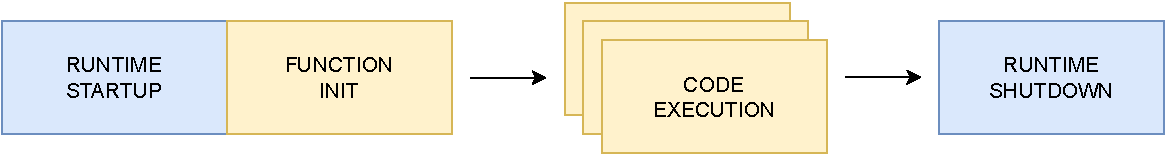
\includegraphics[width=\textwidth]{diagrams/lambda}
  \caption{Serverless function lifecycle in a warm execution environment.}
  \label{fig:serverless-functions-lifecycle}
\end{figure}

\subsection{Serverless principles}

Serverless is a misnomer, since servers are still in the picture,
this computing model must not be confused with other paradigms
that do not require an actual server such as peer-to-peer (P2P)~\cite{serverless-wikipedia}.
Instead, it is more accurate to interpret it as "less-server",
therefore emphasizing the shift in architectural responsibility from developers actively
managing server infrastructure to entrusting platform providers to manage the underlying server complexities.

Figure~\ref{fig:serverless-functions-lifecycle} shows that serverless functions
are ephemeral, so they are designed to have a temporary nature, and consequently
stateless, so there is no stored information of previous transactions, as they are constructed
from scratch each time they are instantiated.
These behaviors have several implications that may offer advantages and disadvantages.

\subsubsection{Serverless architectures benefits}

\paragraph{\textbf{Reduced costs}} Serverless at its core gives immediate
business value to its users, because it outsources servers management
to a vendor, also allowing for economies of scale to take place, as discussed in \cite{berkeley}.
Operational expenses decrease significantly, and development costs are optimized
since this cloud paradigm offers the most fine-grained billing model in which developers
only pay for the actual functions' execution time and not for idle servers.

\paragraph{\textbf{Elasticity}} The cloud provider is responsible for autoscaling the capacity
on demand, hence resources are handled accordingly to accommodate the required load.
For example, consider a web application with two HTTP endpoints, denoted as endpoint $A$ and endpoint $B$,
where $A$ is frequently called while $B$ is very rarely requested.
In a traditional monolith, the entire web app would need to manually be scaled
to handle unpredictable load spikes of $A$ calls, and even in normal circumstances
resources would still be inefficiently allocated just to manage some occasional $B$ requests.
By encapsulating their logic inside two different serverless functions,
endpoint $A$ can be allocated more resources when it experiences high demand,
while endpoint $B$ might cost almost zero due to its occasional requests.

\paragraph{\textbf{Productivity}} Developers can focus solely on writing
business logic. Exposing units of code only through an event-driven model simplifies back-end development,
also alleviating the typical problems related to distributed systems (e.g., multithreading).
Moreover, development becomes quicker as deploying is easier and updates are granular,
thus increasing the agility of the team and rapid prototyping of new products.

\paragraph{\textbf{High availability}} Thanks to the distributed nature of serverless computing,
platform providers ensure fault tolerance by redirecting functions across healthy and available zones.
Latency is also reduced by deploying functions geographically near the end-users.

\paragraph{\textbf{Interoperability}} The serverless paradigm can be used in
conjunction with code deployed in traditional styles,
such as microservices or monoliths~\cite{serverless-wikipedia}.
Therefore, this model can be incrementally adopted by large companies and benefit
complex existing systems. Though, start-ups should prioritize following a pure serverless approach
because of all the previously mentioned benefits.

\subsubsection{Serverless architectures shortcomings}

Serverless computing is not flawless, and some researchers \cite{two-steps-back}
point out the limits that are inherent to this paradigm, which cannot be solved
by updating the state of the art even with tools like \f{}.

\paragraph{\textbf{State management}} Considering that there is no server-state,
the programming model needs to shift for developers, as numerous applications require
storing data for future references.
To limit this disadvantage, users may use:
\begin{itemize}
  \item Temporary data stores or distributed caches, like Redis.
  \item Databases, both SQL or NoSQL, as long as the connections can be instantiated quickly.
  \item Vendor-specific strategies, like \textit{AWS}' step functions or \textit{Azure}'s durable functions.
\end{itemize}
Also, the limited lifetime of serverless functions needs to be contemplated given that
they are not designed to support long-running processes,
and if misused they can become more costly than traditional solutions.

\paragraph{\textbf{Cold starts}} Serverless functions startup times
can be a crucial drawback for systems performance, as the overhead for
allocating all the resources needed to run a function can cause significant
delays. This well-known problem, named "cold start", is
particularly emphasized with technologies requiring heavy runtimes, such as \textit{JVM}-based languages.
To avoid this constraint, platform providers usually wait some time
before dismantling the container, keeping it in a so-called "warm" state, as shown in Figure~\ref{fig:serverless-functions-lifecycle},
so they are able to run the code without all the initialization overhead:
this approach is obviously more costly, but it dramatically improves performances.

\paragraph{\textbf{Vendor lock-in}} Any outsourcing strategy is subject to this limitation.
Users are bound to the vendors' decisions who wield control over
system downtimes, cost changes, loss of functionality, forced API upgrades and many
more limits that may, at times, be enforced unilaterally.
In addition, each vendor offers different features and workflows,
often deeply integrated with their own private services,
and as a result switching vendors means updating operational tools (deployment, monitoring, etc.),
modifying the code to satisfy the new FaaS interfaces, and most importantly
porting chunks of the architecture from one infrastructure to another.
To circumvent these issues, programs should be created in platform-agnostic manner,
without relying too heavily on the third-party services offered by the platform provider.
Moreover, serverless architectures can be achieved through open-source solutions
at the expense of self-hosting parts of the infrastructure.

\paragraph{\textbf{Complex debugging}} Monitoring, tracing, logging, and debugging
are harder in serverless environments because of their ephemeral and stateless nature.
These limits originate from the fact that that cloud environments are difficult
to simulate in local contexts, therefore even techniques like integration testing become unpractical.
Although entire functions can be timed, there is typically no
ability to dig into more detail by attaching profilers, debuggers or APM tools \cite{debug}.

\subsection{Serverless use cases}

A meta-analysis conducted by Eismann et al.~\cite{meta-analysis} reviewed
89 real-world use cases of serverless architectures and studied their characteristics.
Their findings provide insightful values on how this
paradigm is being used and how well it performs:
\begin{itemize}
  \item \textit{AWS Lambda} is the most popular platform provider, taking up 80\% of the market share:
    this is not surprising as they pioneered the most mature and well integrated set of services out of all
    the cloud vendors.
  \item \textit{JavaScript} and \textit{Python} are the most used
    programming languages for cloud functions (each used by 32\% of the cases).
    Most of these architectures depend on a wide variety of cloud services, with the most used
    ones being cloud storage, cloud database, API gateway and cloud pub-sub.
  \item Cost savings seem to be the strongest motivator for adopting serverless computing,
    still, other driving factors are reduced operation effort, the scalability and performance gains.
  \item The overall trend of serverless workloads is to feature unpredictable on-demand
  workloads, typically triggered through lightweight (<1MB) HTTP requests.
\end{itemize}

The first two points also serve to understand how \f{} operates:
we chose to compile \textit{JavaScript} codebases written following
\textit{AWS Lambda}'s interfaces due to their ever-growing popularity.
Furthermore, the meta-programming offered through \f{}'s annotations
can be expanded to support different platform providers.

To simplify the development of serverless architectures even more,
\f{} not only manipulates source codes, but it also generates metadata used
by the \textit{Serverless Framework} \cite{sls} (referred to as \textit{SLS} in this thesis):
this framework streamlines the operational efforts by providing a simple abstraction layer
that can deploy with ease to all major cloud providers by tweaking a few configuration details.
Thus, \textit{SLS} helps in breaking the shortcomings of vendors' control, and it also brightens
the developer experience by extending workflows through CLI tools, debugging facilities and useful plugins.

\section{Server-side JavaScript}
\label{sec:node}

\begin{quote}
  \textit{"Any application that can be written in JavaScript, will eventually be written in JavaScript."}
\end{quote}

As time passes, this quote by Jeff Atwood becomes more and more accurate:
in fact, it should be expanded in scope to include all types of software,
as \textit{JavaScript} continues to evolve and keeps being one of the most
popular programming languages of all time.

Despite its humble beginnings, its versatility and simplicity
have taken the language a long way, giving rise to a vibrant open-source ecosystem
that has enlarged its domain beyond web browsers:
\textit{JavaScript} is now widely used in diverse fields including
game development, IoT, data analysis, and numerous other contexts.

Probably, the most important contribution to the language has been
the advent of \textit{Node.js} in 2009 \cite{node}, which is a runtime environment
that executes \textit{JavaScript} outside a web browser.
This technology played a pivotal role in reshaping users' perceptions of \textit{JavaScript}:
it transitioned from being regarded as a mere scripting language
to being recognized as a capable general-purpose one.

\textit{Node.js} stands apart from traditional programming language runtimes,
and, instead, inherits the strengths of \textit{JavaScript} and builds upon them,
making this environment unique in many ways.
\textit{Node.js} operates on a single-thread event loop,
using non-blocking I/O calls, allowing it to support tens of thousands
of concurrent connections without incurring the cost of thread context switching.

This event-driven design optimizes throughput and scalability in architectures
bound to many asynchronous I/O operations, but it is limited in CPU-heavy environments
given the single-threaded nature of \textit{Node.js}.
For this reason, \textit{Node.js} shines in serverless architectures more than
traditional ones, since it is a great runtime to write the ephemeral and stateless
cloud functions, where users do not need to think about the orchestration of distributed systems.

\subsection{TypeScript}

\textit{TypeScript} is a superset of \textit{JavaScript} with an additional fundamental layer: the type system.

Just like \textit{Node.js}, \textit{TypeScript} is a pretty unique technology.
Indeed, this language was born to fix many of the quirks present in \textit{JavaScript},
which, given its popularity, started being used in codebases with hundreds of thousands of lines of code,
even though, it was never intended for such use cases, hence,
its error-prone nature started appearing at runtime with all its oddities and surprises.
While other tools tried replacing it, and consequently failed (e.g., \textit{CoffeeScript}),
\textit{TypeScript} embraced it and added a compile-time type checker to drastically lower the chance of bugs.

\textit{TypeScript} is a strongly typed programming language,
but it is also designed to support existing \textit{JavaScript} codebases,
and as a result many of the strict type checks performed can be loosened up to
compile regular \textit{JavaScript}. Furthermore, \textit{TypeScript} guarantees
to preserve the runtime behavior, even if the compiler raises type errors,
allowing the transition between the two languages to happen without subtle differences.
Once the compiler has finished checking the code, the types are erased and the resulting
code has no type information.

Normally, \textit{TypeScript} is very strict during its checks,
so other than blocking the weird \textit{JavaScript} parts,
it also provides guards for writing code at enterprise level,
ensuring that everything works even in big projects with multiple teams,
as long as the established type definitions are followed.

\begin{lstlisting}[language=javascript, caption={\textit{TypeScript}'s type checks}, label={lst:ts-checks}]
/* Guards against JavaScript's quirks */
if ('' == 0) {
}
// Error: This comparison appears to be unintentional because the
// types 'string' and 'number' have no overlap.

console.log(4 / [])
// While this is a syntactically-legal instruction that logs `Infinity`,
// TypeScript will issue an error because it is a nonsensical operation.

/* Strict type checks */
type User = {
  firstName: string
  lastName: string
  role: 'Professor' | 'Student'
}

const user: User = {
  firstName: 'Angela',
  lastName: 'Davis',
  role: 'Professor',
  name: 'Angela Davis',
}
// Error: Object literal may only specify known properties
// and 'name' does not exist in type 'User'.
\end{lstlisting}

Listing~\ref{lst:ts-checks} previews a very important principle of \textit{TypeScript},
its structural type system. Although, most strongly typed languages implement a nominal type system,
where two types are considered equal when their names correspond,
\textit{TypeScript} had to be more pervasive to enhance
\textit{JavaScript}'s dynamic duck typing \cite{duck-typing},
and as a consequence it implements structural checks, where, rather than the name,
the shapes of the values are compared.

\begin{lstlisting}[language=javascript]
type Dollar = number
type Euro = number
function foo(n: Dollar)
let e: Euro
// This function call raises an error in a nominal system
// because `foo` only accepts an argument of type `Dollar`,
// but works completely fine in a structural system,
// since the two types share the same shape of `number`.
foo(e)
\end{lstlisting}

To be more precise, \textit{TypeScript}'s type system is not entirely structural,
as it offers nominal typing-like mechanisms to simplify the writing of new definitions,
by making types unique symbols across their contexts, which is especially useful for
creating recursive data structures.

All these key factors (i.e., strictness, compatibility with \textit{JavaScript}, structural typing),
have greatly boosted \textit{TypeScript}'s popularity at every scale of software development.
On top of that, it introduces powerful features that improve developers' experience:

\begin{itemize}
  \item Types inference support vastly superior in comparison to most of the commercial
    general-purpose programming languages.%, also including flow-sensitive typing.
  \item Enriched build pipeline. Before \textit{TypeScript} existed, projects
    were developed through complex combinations of different tools, especially if the
    developers preferred to use newer features of \textit{JavaScript} that were not
    supported by the runtime yet. \textit{TypeScript} simplifies these workflows since it provides
    an inclusive build system which compiles even the experimental features of the language
    to older versions without the need for polyfills or other technologies.
  \item Better tooling through open-source contributions.
    For example, \textit{TypeScript} was the reason behind the birth of the \textit{Language Server Protocol} (\textit{LSP}),
    which enriches code editors with language intelligence tools such as code completion, syntax highlighting,
    error marking, refactoring routines and many more features. Traditionally, all this work
    had to be repeated for each programming language as they all built upon different APIs,
    but now all major programming languages follow this specification, which decouples
    the language services from the editors.
    This is just one of the tools built because of and for \textit{TypeScript},
    but it should not be underestimated since it improves developers' experience significantly.
\end{itemize}

In serverless computing, where functions need to be self-contained, concise, and easily deployable,
\textit{TypeScript} strengths are particularly valuable, since
it encourages developers to write robust and maintainable code.
This is convenient since cloud functions are harder to test and debug,
and having compile-time errors reduces maintenance costs and saves a lot of time.

\f{} uses the parser offered by the \textit{TypeScript} API
to handle AST traversals and manipulations,
so it parses both \textit{TypeScript} and \textit{JavaScript} codebases.
